\documentclass[xcolor={dvipsnames},pdf, hyperref={colorlinks=true, citecolor=ForestGreen, linkcolor=BlueViolet, urlcolor=Magenta}]{beamer}
\usetheme{Frankfurt}  
\usecolortheme{whale}
\usepackage{tikz} 
\usepackage{amsmath}
\usepackage{amsthm}
\usepackage{amssymb}              % used for \eqref{} in this document
\usepackage{dsfont}
\usepackage{hyperref}
\usepackage{threeparttable}
\usepackage{multirow}
\graphicspath{{Figures/}}
\usepackage{booktabs}
\usepackage{tikz}
\newtheorem{exmp}{Example}[section]
\usepackage{subcaption}
\usepackage{adjustbox}
\usepackage{graphicx}
\usepackage[mathscr]{euscript}
\usepackage{remreset}% tiny package containing just the \@removefromreset command
\makeatletter
\@removefromreset{subsection}{section}
\makeatother
\setcounter{subsection}{1}
\usepackage{float}
\usepackage{sgamevar}
\usepackage{sgame}


\newcommand{\defn}[1]{\textbf{#1}}


%Instructor version
\newcommand{\blank}[0]{}
\newcommand{\ddp}[1]{{\textcolor{ForestGreen}{#1}}} 
\newcommand{\dd}[1]{{\underline{\textcolor{ForestGreen}{#1}}}}

%Student version
%\newcommand{\blank}[0]{\vspace{2em}}
%\newcommand{\dd}[1]{\underline{\hspace{3cm}}} 
%\newcommand{\ddp}[1]{}

\addtobeamertemplate{navigation symbols}{}{%
	\usebeamerfont{footline}%
	\usebeamercolor[fg]{footline}%
	\hspace{1em}%
	\insertframenumber/\inserttotalframenumber
}

\section{Price Ceilings}

%% preamble
\title{Price Controls and Taxes}
\author{David A. D\'iaz }
\institute{UNC Chapel Hill}
\date{}

\AtBeginSection[] %Section links on slides

\begin{document} 
	
	\begin{frame}
		
		\titlepage
		
	\end{frame}
	
\begin{frame}{Government Policy}
	\begin{itemize}
		\item 	The focus of this section is to analyze different types of government policies using the tools of supply and demand. 
		\item We will also look at the welfare implications of these policies.
		\item We will assume that markets do not have any positive or negative externalities.
		\item Under this assumption, we will see that government intervention in markets will \textit{reduce} total surplus and is thus inefficient.
		\item Next time, we will see that in certain cases (e.g., in markets with externalities), government policy is necessary in order to maximize surplus.
	\end{itemize}

\end{frame}

\begin{frame}{Price  Ceilings}
	\begin{itemize}
		\item 	\defn{Price ceiling:} A legal maximum on the price at which a good can be sold.
		\item Consider two types of price ceilings, one that is above the market price and one that is below:
		\blank\blank\blank\blank
		\begin{figure}[H]
			\centering
			\ddp{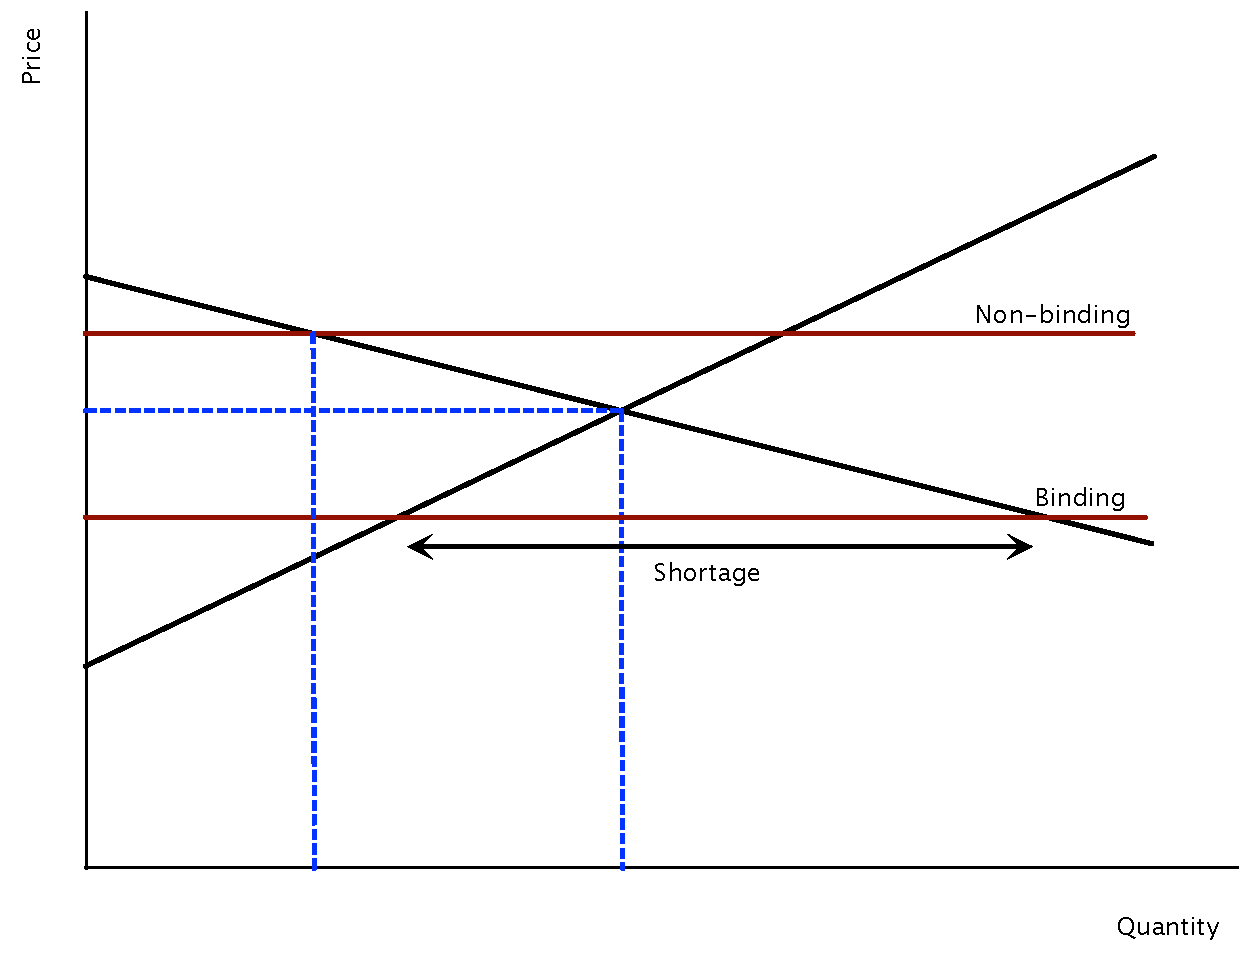
\includegraphics[scale=.30]{plot34.pdf}}
			\caption{Price Ceilings}
		\end{figure}
	\end{itemize}
\end{frame}

\begin{frame}{Price  Ceilings}
	\begin{itemize}
		\item If the government sets a price ceiling above the market price, then the ceiling is \dd{non-binding}.
		\item If the government sets a price ceiling below the market price, then the ceiling is \dd{binding}.
	\end{itemize}
\end{frame}

\begin{frame}{Price  Ceilings}
	\begin{itemize}
		\item Market forces move the economy towards the equilibrium point where $Q_d = Q_s$.
		\item In the case of a binding price ceiling, once the price in the market hits the ceiling it cannot increase any further by law.
		\item Therefore, if the price ceiling is binding, the market price equals the price ceiling.
	\end{itemize}
\end{frame}

\begin{frame}{Price  Ceilings}
	\begin{itemize}
		\item At this price, we have that \dd{$Q_D$} is greater than \dd{$Q_S$}. Thus, there is a \dd{shortage}.
		\item Due to this shortage, some mechanism for rationing will develop. Two potential ones are
		\begin{enumerate}
			\item \ddp{Long lines}
			\item \ddp{Rationing according to seller bias}
		\end{enumerate}
	\item Both types of rationing mechanisms above are not \dd{efficient}. 
	\ddp{
			\begin{enumerate}
				\item Long lines waste time
				\item Seller bias: goods do not necessarily go to the buyer that values it most
			\end{enumerate}}
	\item On the other hand, free markets ration goods with \dd{prices}. This mechanism is both \dd{efficient} and \dd{impartial}.
	\end{itemize}
\end{frame}

\begin{frame}{Price Ceilings}
	\begin{exmp}
		\scriptsize
		A recent study found that the demand and supply schedules of Frisbees are as follows (quantities are in millions):
		\begin{table}[H]
			\caption{Supply and Demand for Frisbees}

			\centering
			\begin{tabular}{ c|c|c}        
				Price   & $Q_D$ & $Q_S$\\
				\hline
				\$11 & 1 & 15 \\
				\$10 & 2 & 12 \\
				\$9 & 4 & 9 \\
				\$8 & 6 & 6 \\
				\$7 & 8 & 3 \\
				\$6 & 10 & 1 \\
			\end{tabular}
		\end{table} 
	\begin{enumerate}
		\item What is the equilibrium price and quantity of Frisbees? \pause \ddp{$P^* = 8, Q^* = 6$}
		\item Under pressure from worried college students, officials in Washington pass a law that stipulates the price of Frisbees cannot rise higher than \$6. What is the new market price? How many Frisbees are sold? \pause \ddp{$P_C = \$6, Q_C = 1$}
	\end{enumerate}
	\end{exmp}

\end{frame}

\begin{frame}{Price Ceilings}
	\begin{itemize}
	\item 	Consider a market before the introduction of a binding price ceiling and afterwards:
	\begin{figure}[H]
		\centering
		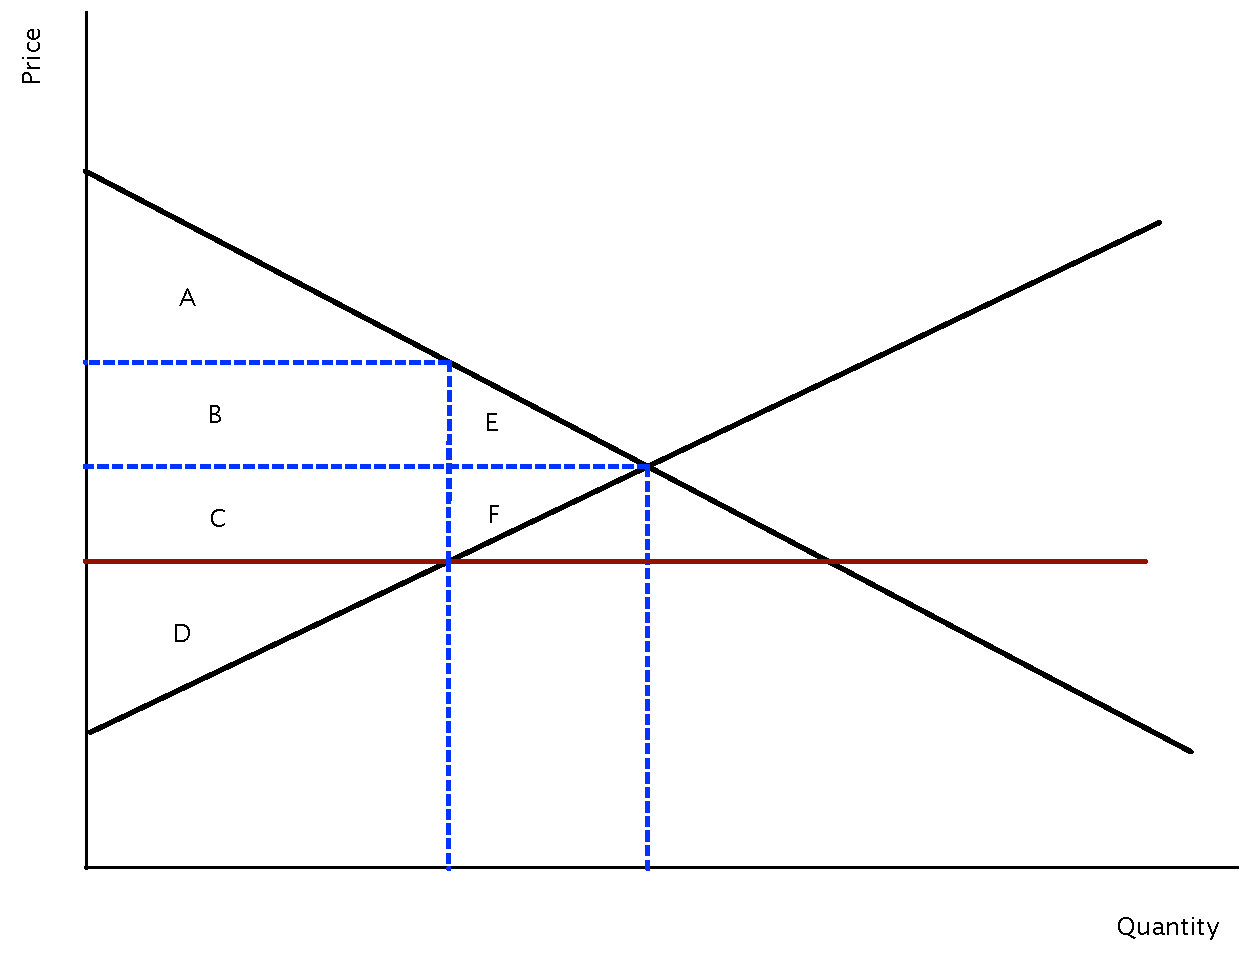
\includegraphics[scale=.35]{plot36.pdf}
		\caption{Price Ceilings and Welfare}
	\end{figure}
\end{itemize}
\end{frame}

\begin{frame}{Price Ceilings}
\begin{itemize}
	\item 	Before the introduction of the ceiling, buyers and sellers were paying and receiving price $P^*$. Thus, 
	\begin{align*}
	\text{CS}_0 &= \ddp{A + B + E}\\
	\text{PS}_0 &= \ddp{C + D + F}\\
	\text{TS}_0 &= \ddp{A + B + C + D + E + F}
	\phantom{\hspace{9cm}}
	\end{align*}
\end{itemize}
\end{frame}

\begin{frame}{Price Ceilings}
\begin{itemize}
	\item 	After the price ceiling is introduced, the market price is $P_c$. Buyers and sellers are now paying and receiving \dd{less} than before. Moreover, the number of transactions that are taking place has \dd{decreased}. Now, 
	\begin{align*}
	\text{CS}_1 &= \ddp{A + B + C}\\
	\text{PS}_1 &= \ddp{D}\\
	\text{TS}_1 &= \ddp{A + B + C + D}
	\phantom{\hspace{9cm}}
	\end{align*}
\end{itemize}
\end{frame}

\begin{frame}{Deadweight Loss}
\begin{itemize}
	\item 	This \dd{decrease} in total surplus (the area \dd{E + F}) is referred to as a \dd{deadweight loss}.
	\item \defn{Deadweight Loss (DWL):} The decrease in total surplus that results from a market distortion.
	\item DWL is caused by either \dd{unrealized gains from trade} or \dd{inefficient transactions}.
\end{itemize}
\end{frame}

\section{Price Floors}

\begin{frame}{Price Floors}
	\begin{itemize}
		\item \defn{Price floor:} A legal minimum on the price at which a good can be sold.
		
		\item Consider two types of price floors, one that is above the market price and one that is below:
			\blank\blank\blank\blank	
		\begin{figure}[H]
			\centering
			\ddp{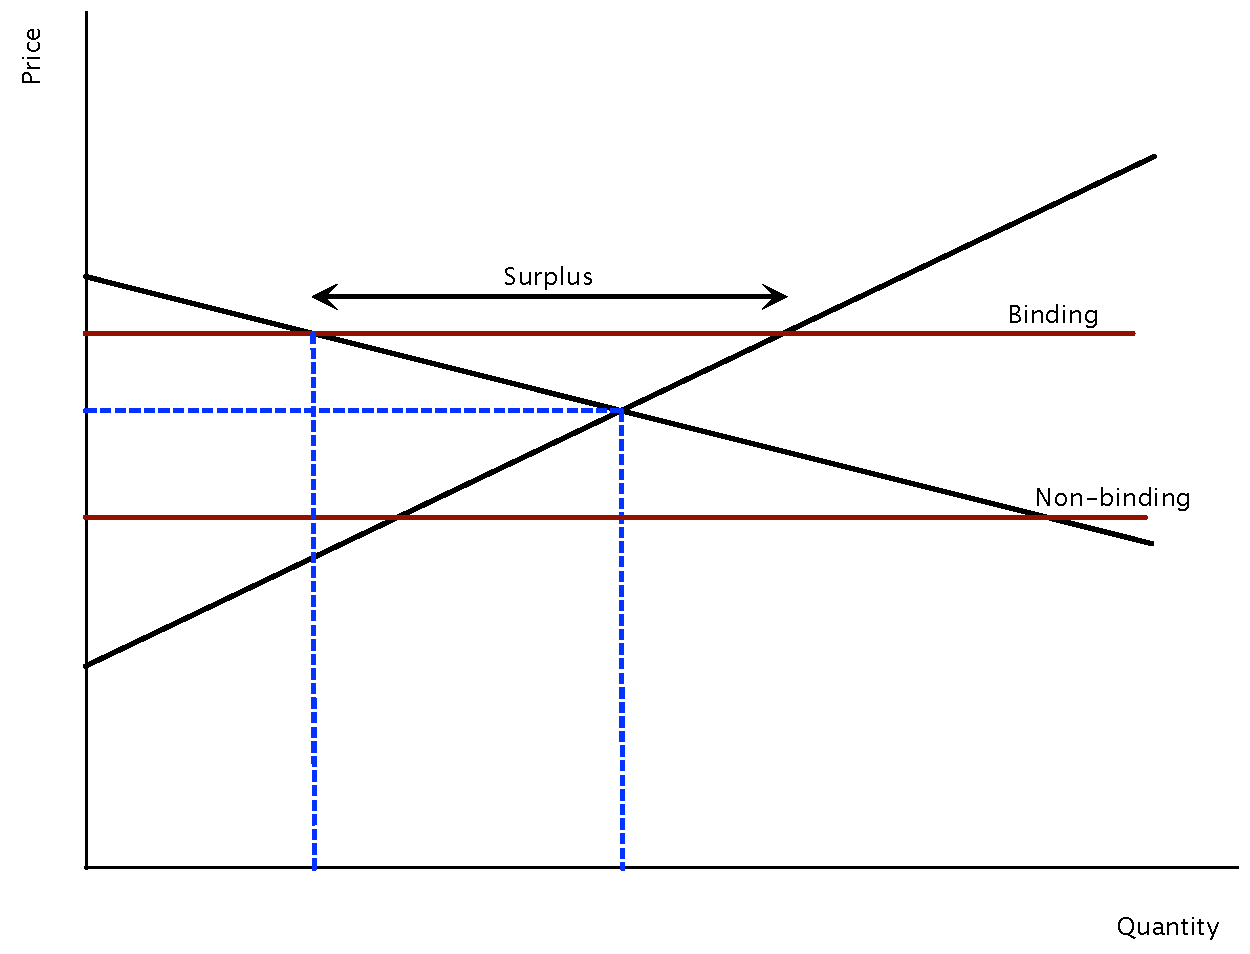
\includegraphics[scale=.30]{plot35.pdf}}
			\caption{Price Floors}
		\end{figure}
	\end{itemize}
\end{frame}

\begin{frame}{Price Floors}
	\begin{itemize}
		\item 	If the government sets a price floor above the market price, then the floor is \dd{binding}.
		\item If the government sets a price floor below the market price, then the floor is \dd{non-binding}.
	\end{itemize}
\end{frame}

\begin{frame}{Price Floors}
	\begin{itemize}
		\item In the case of a binding price floor, once the price in the market hits the floor it cannot decrease any further by law.
		\item  Therefore, if the price floor is binding, the market price equals the price floor.
		\item At this price, we have that \dd{$Q_S$} is greater than \dd{$Q_D$}. Thus, there is a \dd{surplus}.
	\end{itemize}
\end{frame}

\begin{frame}{Price Floors}
	\begin{itemize}
		\item 	Due to this, some mechanism for rationing will develop. Two potential ones are
		\begin{enumerate}
			\item \ddp{Sellers who appeal to personal bias of buyers may be better able to sell the good.}
			\item \ddp{Sellers may try to differentiate by increasing quality (wasteful).}
		\end{enumerate}
	\end{itemize}
\end{frame}

\begin{frame}{Price Floors}
	\begin{exmp}
		\scriptsize
		A recent study found that the demand and supply schedules of Frisbees are as follows (quantities are in millions):
		\begin{table}[H]
			\caption{Supply and Demand for Frisbees}
			
			\centering
			\begin{tabular}{ c|c|c}        
				Price   & $Q_D$ & $Q_S$\\
				\hline
				\$11 & 1 & 15 \\
				\$10 & 2 & 12 \\
				\$9 & 4 & 9 \\
				\$8 & 6 & 6 \\
				\$7 & 8 & 3 \\
				\$6 & 10 & 1 \\
			\end{tabular}
		\end{table} 
	 After the imposition of the \$6 price ceiling, angry Frisbee manufacturers convince the government to impose a price floor \$1 above the former price ceiling. What is the new market price? How many Frisbees are sold? \pause \ddp{The price floor is not binding. $(P^*,Q^*) = (\$8, 6)$}
	\end{exmp}
\end{frame}


\begin{frame}{Application: The Minimum Wage}
	\begin{itemize}
		\item A labor market consists of workers that determine the supply of labor and firms that determine the demand for labor. 
		\item The price of labor is the wage that workers receive and firms pay. 
	\end{itemize}
\end{frame}

\begin{frame}{Application: The Minimum Wage}
	\begin{itemize}
		\item A labor market with a minimum wage above the equilibrium wage (an example of a binding \dd{price floor}) looks like this:
	\blank\blank\blank\blank
			\begin{figure}[H]
				\centering
				\ddp{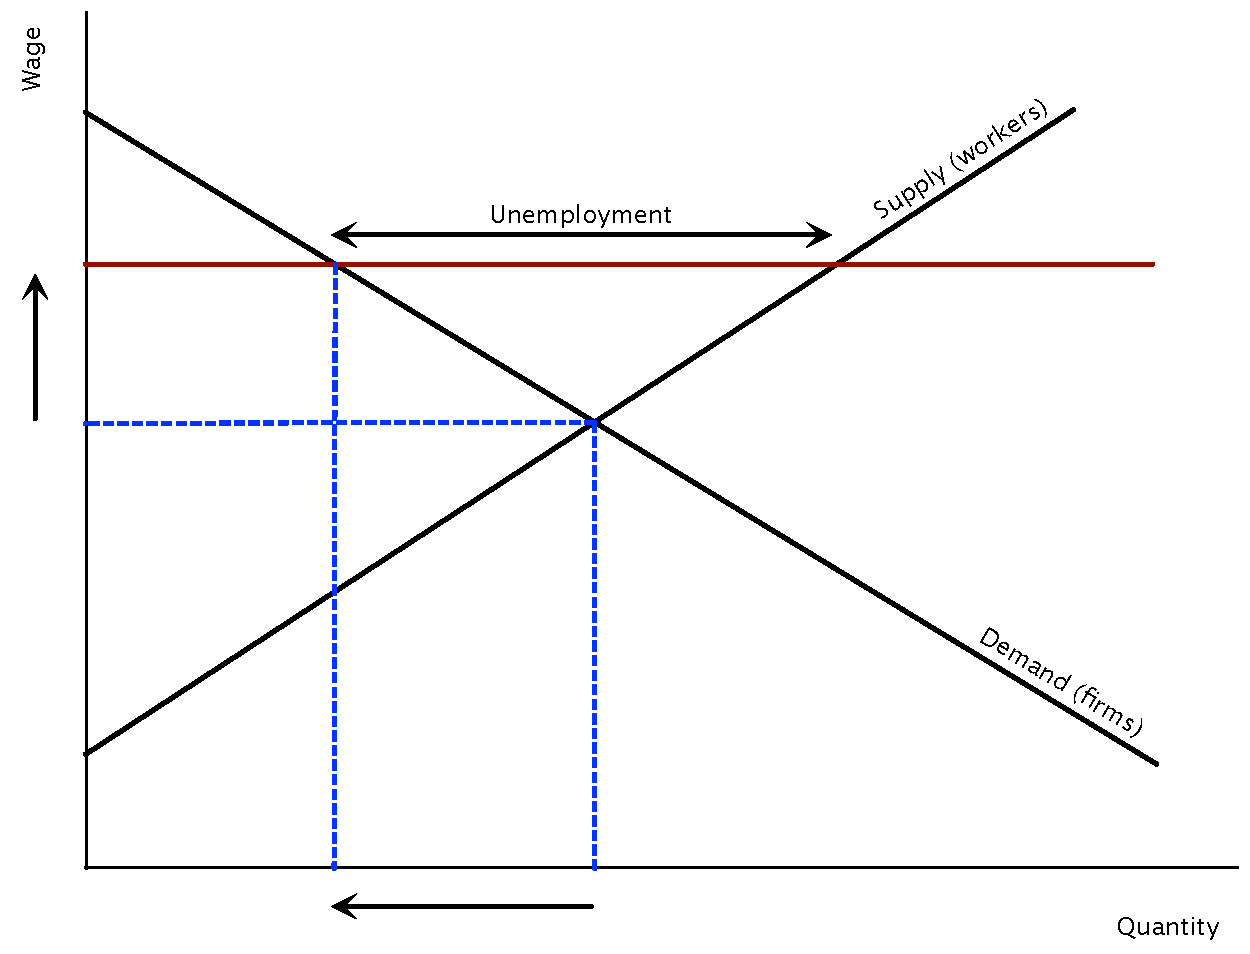
\includegraphics[scale=.25]{plot39.pdf}}
				\caption{Market for Labor}
			\end{figure}
	\item As usual with a binding price floor, there will be a \dd{surplus}. In the market for labor, this is called \dd{unemployment}.
	\end{itemize}
\end{frame}

\begin{frame}{Application: The Minimum Wage}
	
	\begin{exmp} 
		\scriptsize
		Refer to Figure \ref{fig3}. What are the total wage payments made to workers at the equilibrium wage? Suppose a minimum wage of \$8.00 is enacted. What are the total wage payments made to workers in this case?
	\end{exmp}
	\begin{figure}[H]
	\centering
	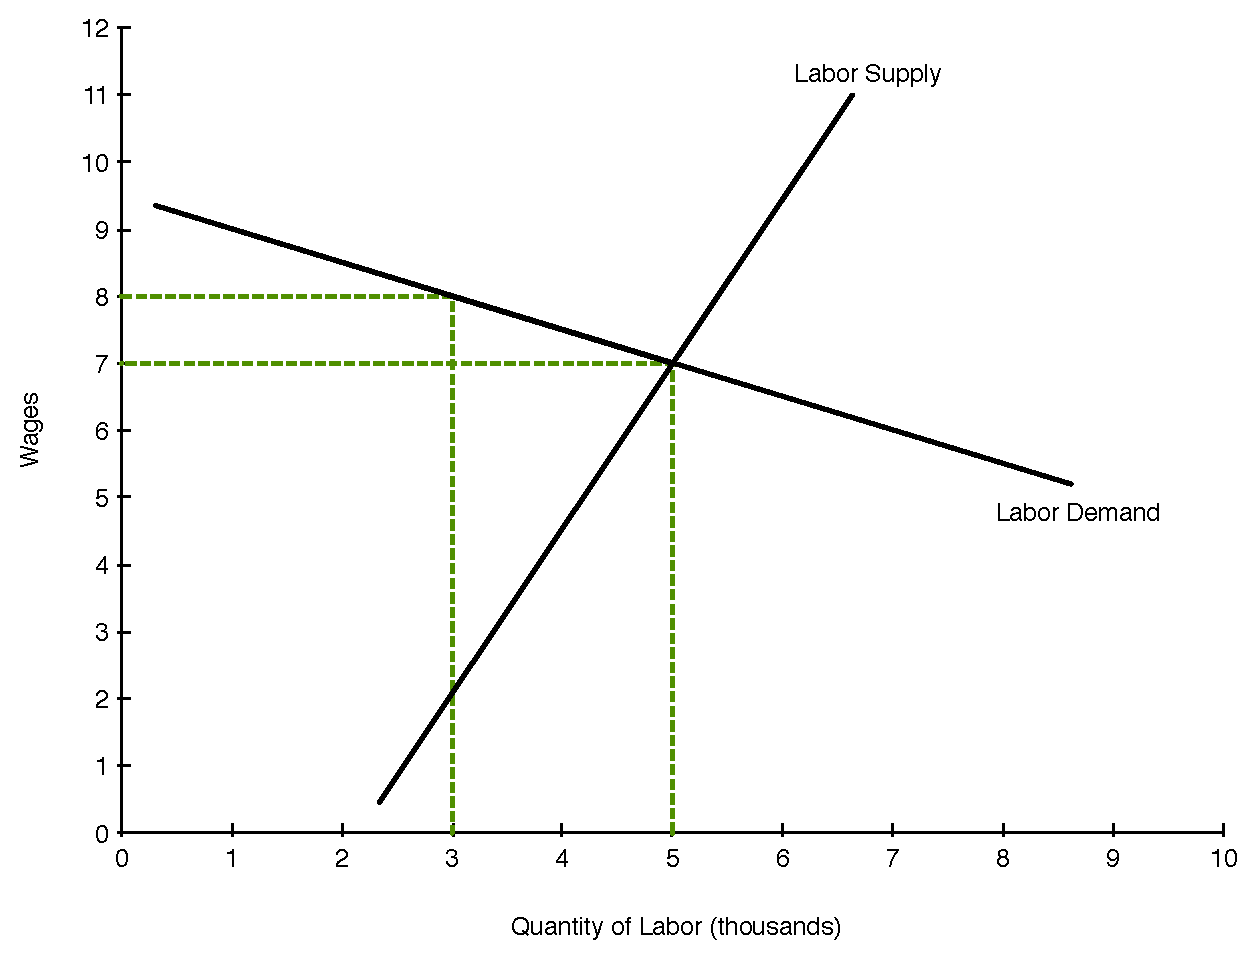
\includegraphics[scale=.24]{notes05_plot1.pdf}
	\caption{Labor Market and Wage Payments}
	\label{fig3}
\end{figure}
	\scriptsize
\pause	\ddp{At eq. wage: $7\times 5,000 = \$35,000$ \\
	At min wage: $8\times 3,000 = \$24,000$.}
\end{frame}

\begin{frame}{Price Floors}
	\begin{itemize}
		\item 	Consider a market before the introduction of a binding price floor and afterwards:
		\begin{figure}[H]
			\centering
		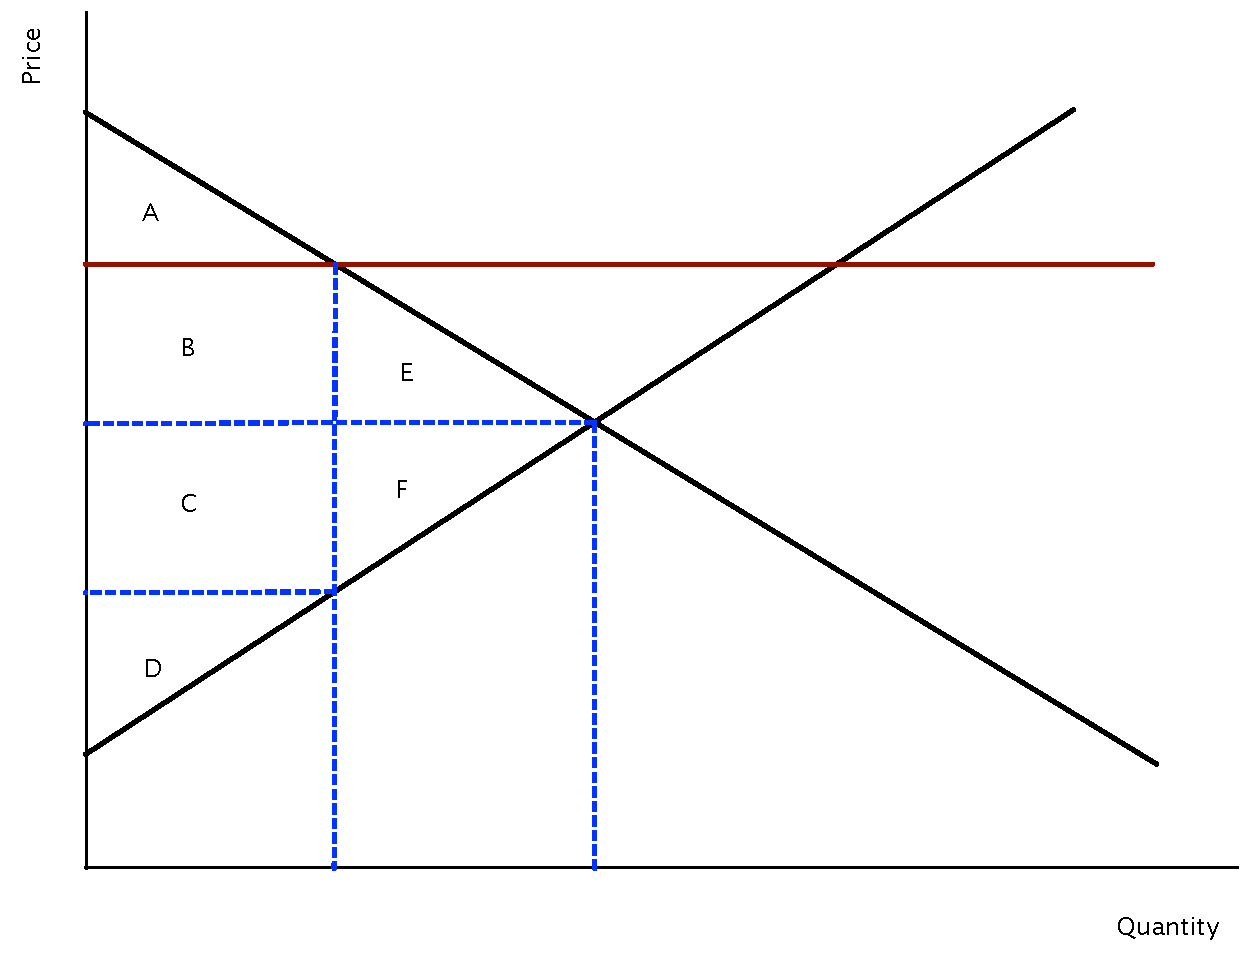
\includegraphics[scale=.35]{plot37.pdf}
			\caption{Price Floors and Welfare}
		\end{figure}
	\end{itemize}
\end{frame}

\begin{frame}{Price Floors}
	\begin{itemize}
		\item 	After the price ceiling is introduced, the market price is $P_f$. Buyers and sellers are now paying and receiving \dd{more} than before. Moreover, the number of transactions that are taking place has \dd{decreased}. Now, 
		\begin{align*}
		\text{CS}_1 &= \ddp{A} \\
		\text{PS}_1 &= \ddp{B + C + D}\\
		\text{TS}_1 &= \ddp{A + B + C + D}
		\phantom{\hspace{9cm}}
		\end{align*}
		\item Again, we see that total surplus decreases due to the price control and the deadweight loss is represented by \dd{E + F}.
	\end{itemize}
\end{frame}

\section{Taxes}

\begin{frame}{Taxes}
	\begin{itemize}
		\item \defn{Tax incidence:} The manner in which the burden of a tax is shared among participants in a market. 
		\item Taxes can be levied on either (1) sellers or (2) buyers. 
	\end{itemize}	
\end{frame}

\begin{frame}{Taxes}
\begin{itemize}
	\item A tax levied on buyers will only affect \dd{demand}. 
	\item The \textit{effective} price buyers pay increases by the size of the tax. 
	\item At any given quantity, the market price must \dd{decrease} by the size of the tax.
	\item Thus, a tax on buyers will \dd{decrease} demand by \dd{exactly} the size of the tax.
	
\end{itemize}
\end{frame}

\begin{frame}{Taxes}
		\begin{figure}
			\centering
		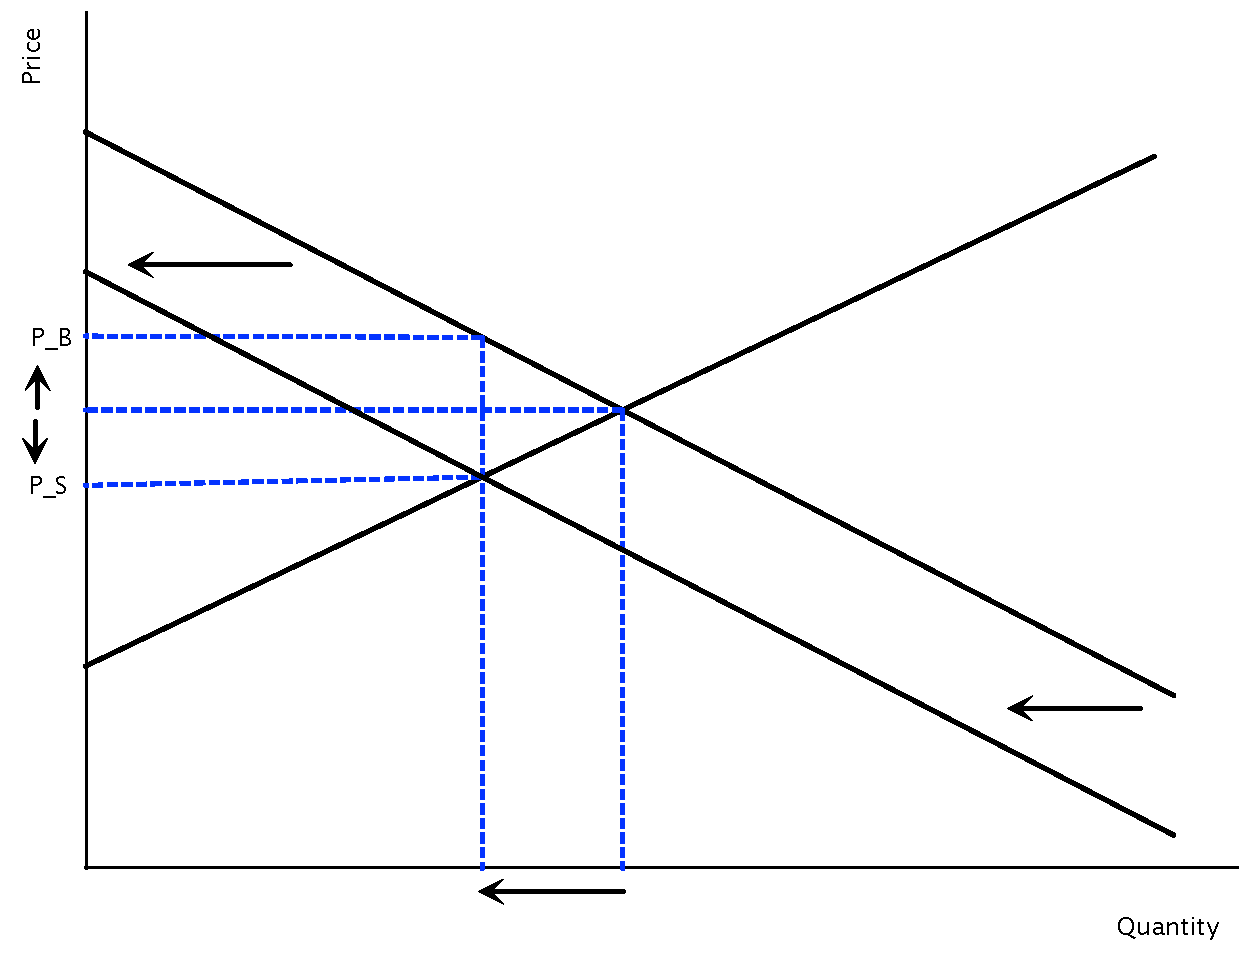
\includegraphics[scale=.30]{plot41.pdf}
			\caption{Tax on Buyers}
		\end{figure}
\end{frame}

\begin{frame}{Taxes}
	\begin{itemize}
		\item A tax levied on sellers will only affect \dd{supply}. 
		\item The \textit{effective} price sellers receive decreases by the size of the tax. 
		\item At any given quantity, the market price must \dd{increase} by the size of the tax.
		\item Thus, a tax on sellers will \dd{decrease} supply by \dd{exactly} the size of the tax.

	\end{itemize}
\end{frame}

\begin{frame}{Taxes}
		\begin{figure}
		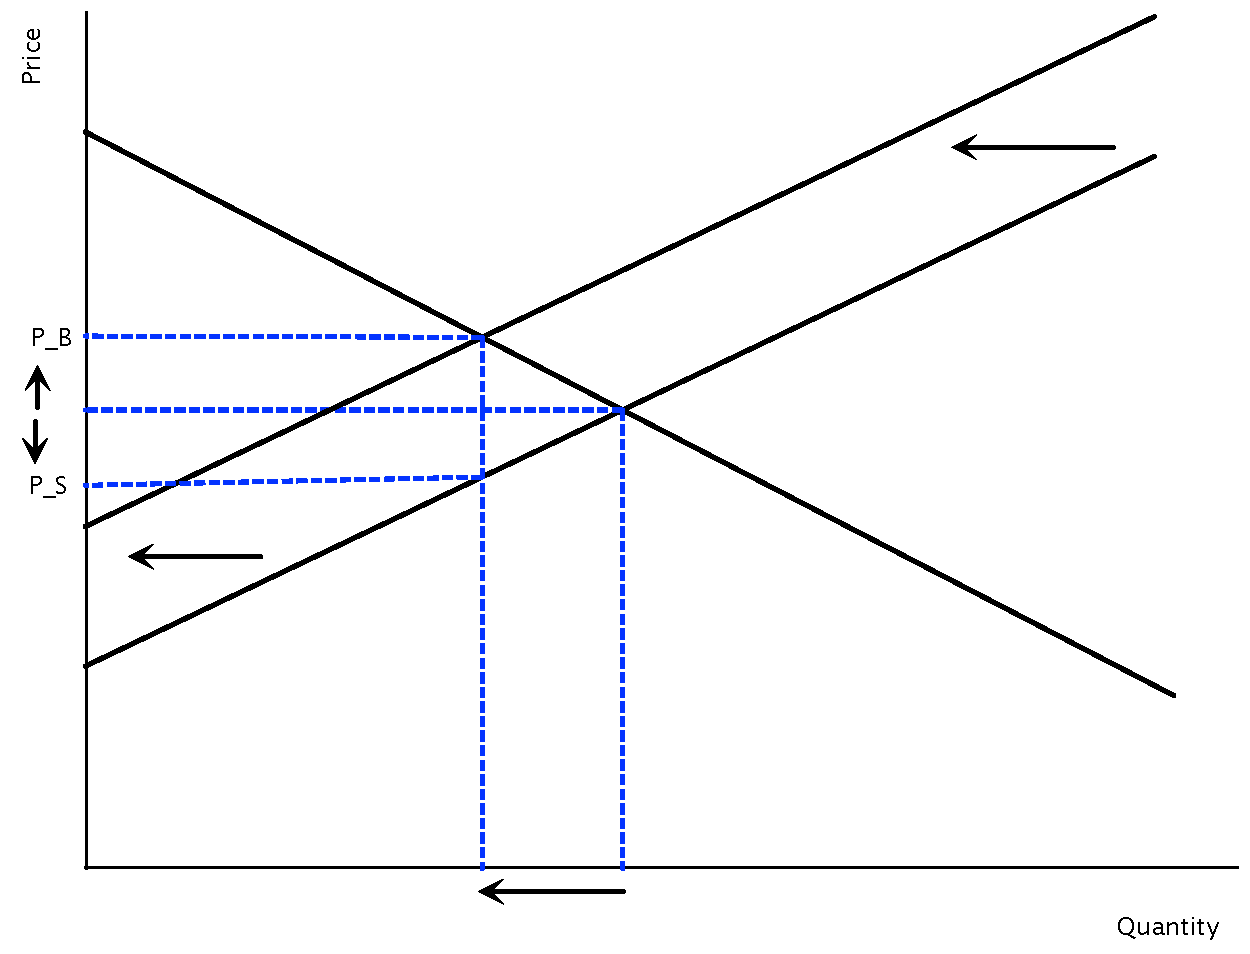
\includegraphics[scale=.30]{plot40.pdf}
			\caption{Tax on Sellers}
		\end{figure}
\end{frame}

\begin{frame}{Taxes}
	\begin{itemize}
		\item Insights:
		\begin{enumerate}
			\item Taxes discourage market activity
			\begin{itemize}
				\item The quantity bought and sold in the market decreases
			\end{itemize}
			\item Buyers and sellers share the burden of taxes. 
				\begin{itemize}
					\item The price buyers pay increases
					\item The price sellers receive decreases
				\end{itemize} 
			\item Taxes levied on buyer and sellers are equivalent
		\end{enumerate}
	\end{itemize}
\end{frame}

\begin{frame}{Taxes}
	\begin{itemize}
		\item The way the burden of the tax is split depends on the relative elasticities of supply and demand. 
		\begin{figure}[H]
			\centering
			\caption{Elasticity \& Tax Incidence}
			\begin{subfigure}{.3\textwidth}
			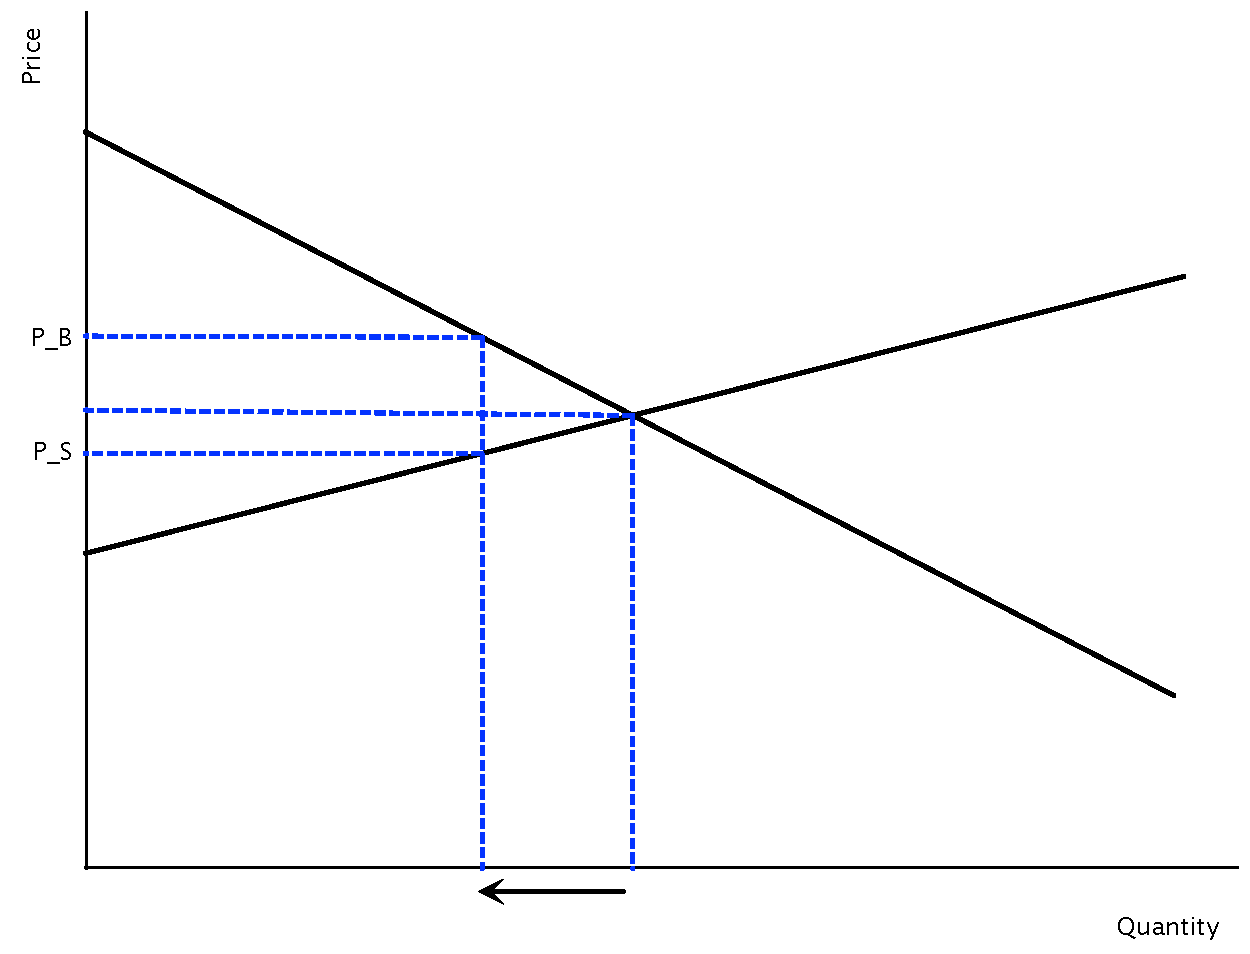
\includegraphics[scale=.2]{plot42.pdf}
				\caption{Elastic Supply}
			\end{subfigure}%
			\begin{subfigure}{.5\textwidth}
				\centering
			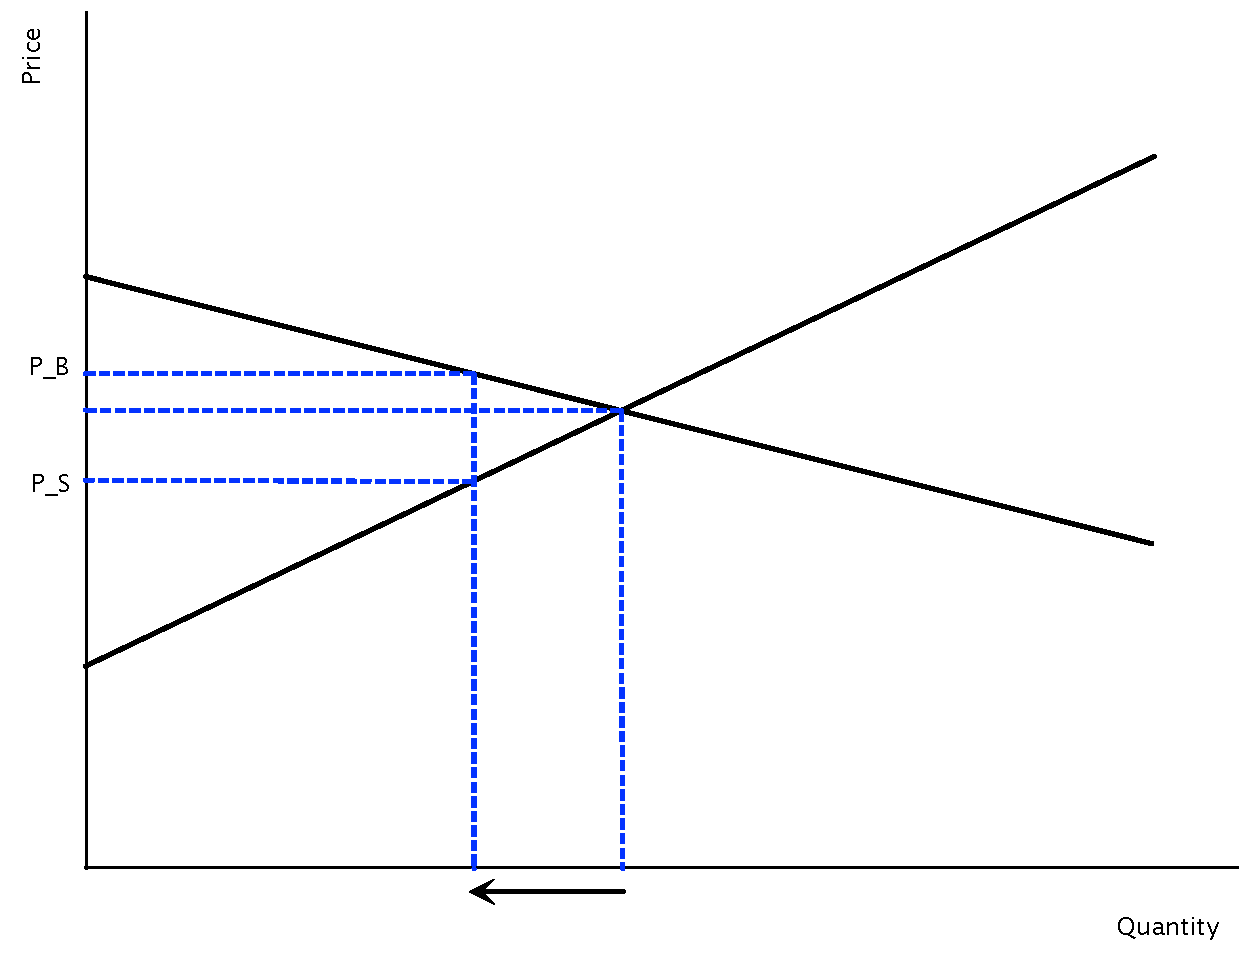
\includegraphics[scale=.2]{plot43.pdf}
				\caption{Elastic Demand}
			\end{subfigure}
		\end{figure}
	\item 	The tax burden falls more heavily on the side that is \dd{less} elastic.
	
	\end{itemize}
\end{frame}


\begin{frame}{Taxes}
	\begin{itemize}
		\item 	When the government levies a tax, it collects \dd{tax revenue}. Though this benefit accrues to those on whom the revenue is spent and not the government itself, we use this to measure the public benefit from the tax. Tax revenue is simply \dd{$\tau \times Q_{\tau}$}. 
		\begin{figure}[H]
			\centering
			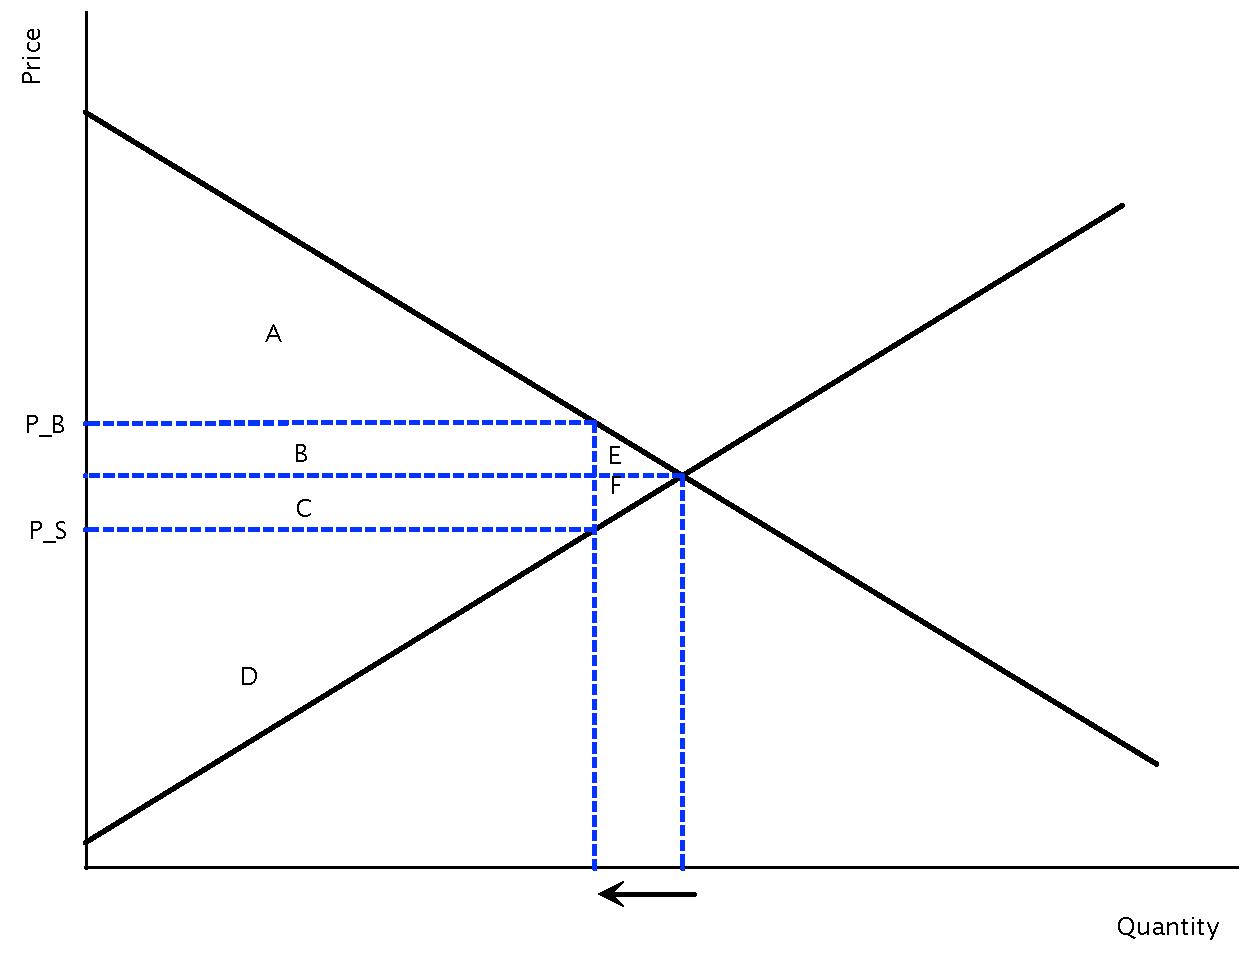
\includegraphics[scale=.3]{plot44.pdf}
			\caption{Taxes and Welfare}
		\end{figure}
	\end{itemize}
\end{frame}

\begin{frame}{Taxes}
	\begin{itemize}
		\item By increasing the price buyers pay and decreasing the price sellers receive, a tax \dd{reduces} consumer and producer surplus. 
		\item Moreover, total surplus \dd{decreases} because the tax revenue earned by the government is \dd{outweighed} by the decreases in CS and PS. Thus, taxes lead to a deadweight loss.
		\item The decrease in total surplus is due to \dd{unrealized gains from trade}.
	\end{itemize}
	
\end{frame}

\begin{frame}{Taxes}
	\begin{itemize}
		\item The driving factor behind the size of the deadweight loss is the \dd{elasticity} of supply and demand. 
	\end{itemize}
	\begin{figure}[H]
		\centering
		\caption{Taxes, Elasticity, and DWL}
		\begin{subfigure}{.5\textwidth}
			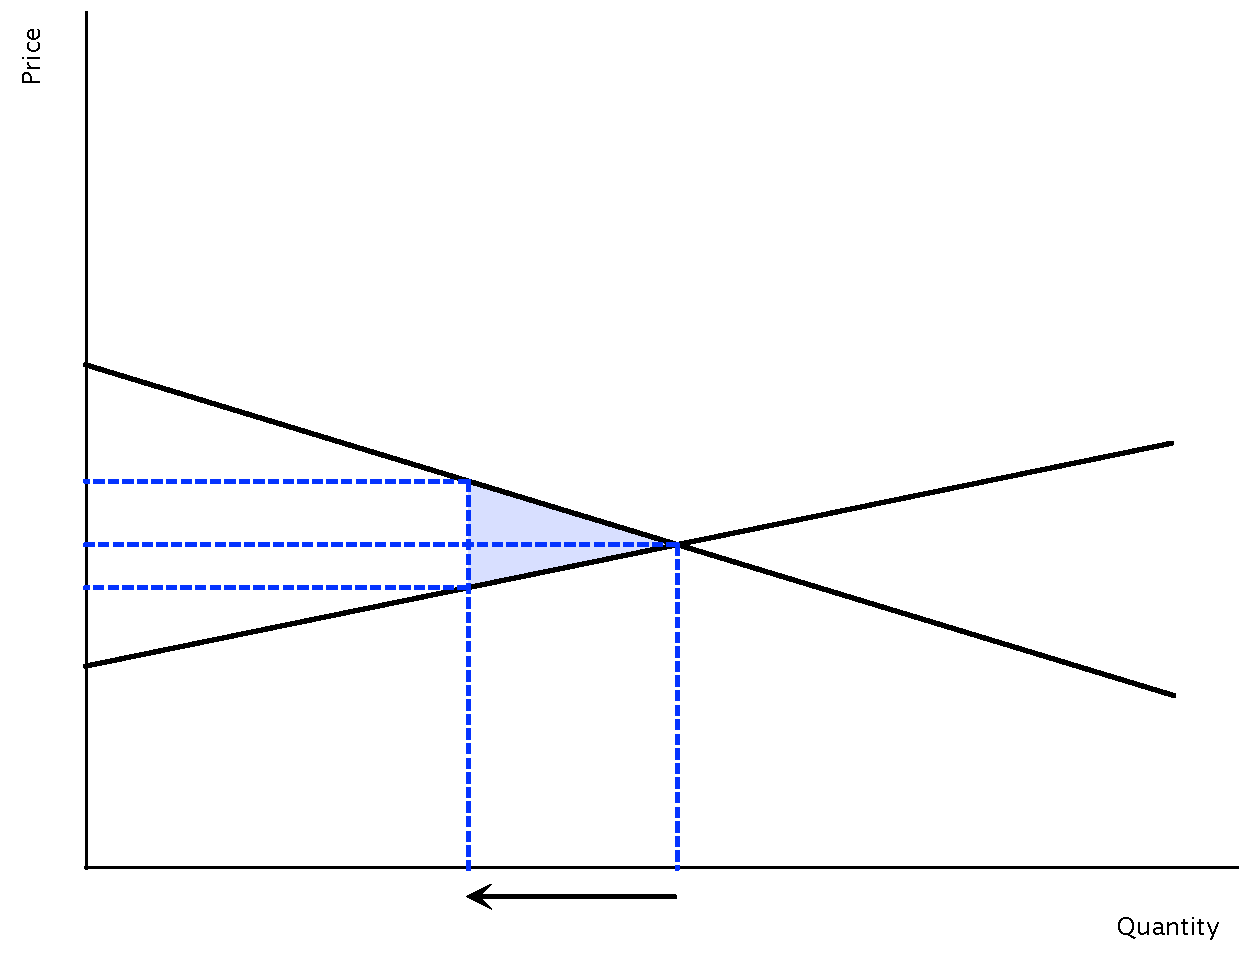
\includegraphics[scale=.25]{plot45.pdf}
			\caption{Elastic Supply and Demand}
		\end{subfigure}%
		\begin{subfigure}{.5\textwidth}
			\centering
		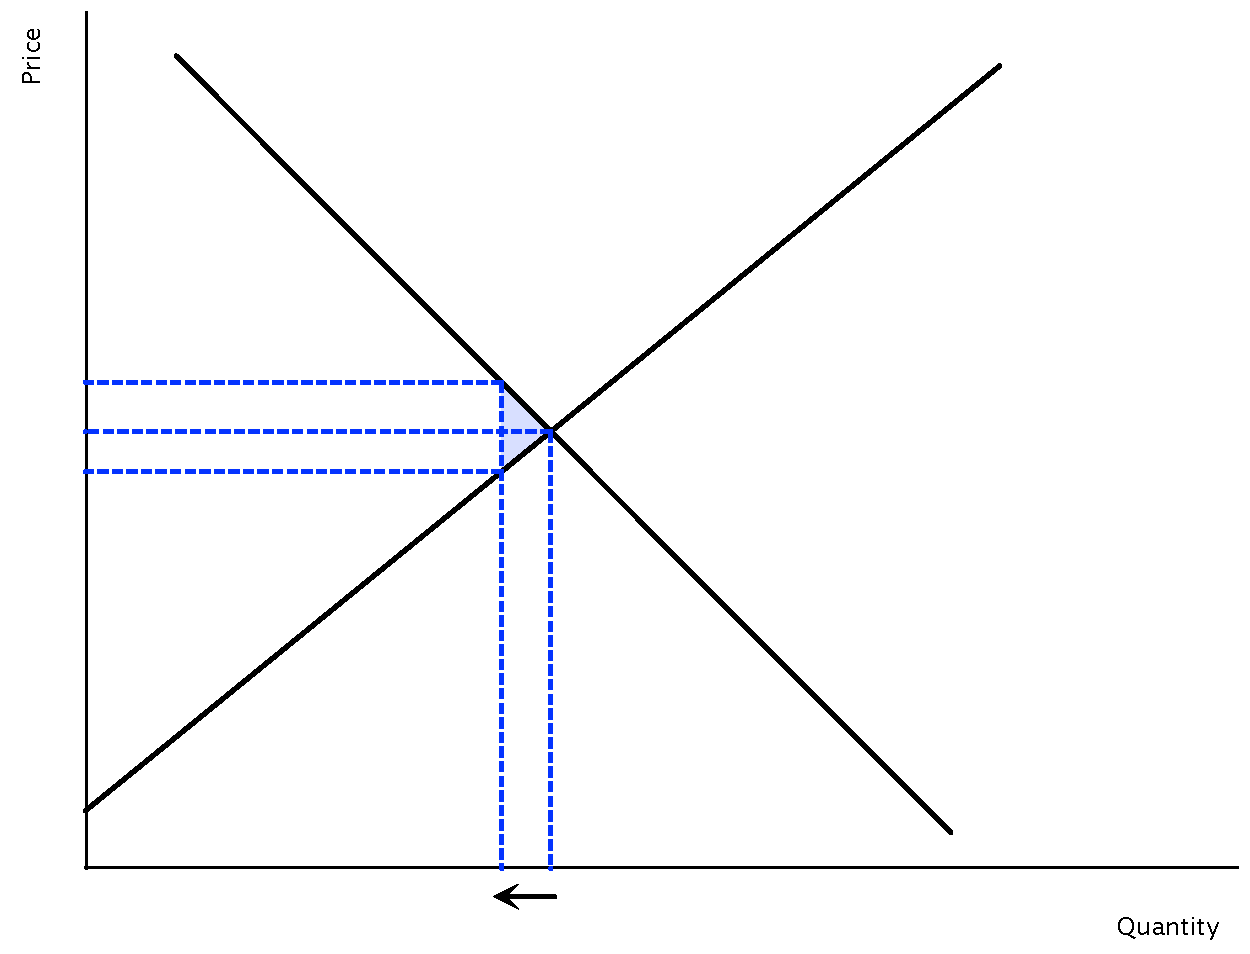
\includegraphics[scale=.25]{plot46.pdf}
			\caption{Inelastic Supply and Demand}
		\end{subfigure}
	\end{figure}
	
\end{frame}

\begin{frame}{Taxes}
	\begin{itemize}
		\item The \dd{greater} the elasticities of supply and demand, the \dd{greater} the DWL of a given tax will be.
		\item Buyers and sellers are more able to move away from the market, so there are fewer transactions taking place. This leads to more unrealized gains from trade.
	\end{itemize}
\end{frame}

\begin{frame}{Taxes}
	\begin{itemize}
		\item 	For a given supply and demand curve, the DWL of the tax always \dd{increases} as the tax increases.
		\item The amount of tax revenue collected \dd{increases} initially as the tax increases, but eventually \dd{decreases} as the tax continues to increase.
	\end{itemize}
	

	
\end{frame}

\begin{frame}{Taxes}

	\begin{figure}[H]
		\centering
		\caption{Taxes, DWL, and Tax Revenue}
		\begin{subfigure}{.3\textwidth}
			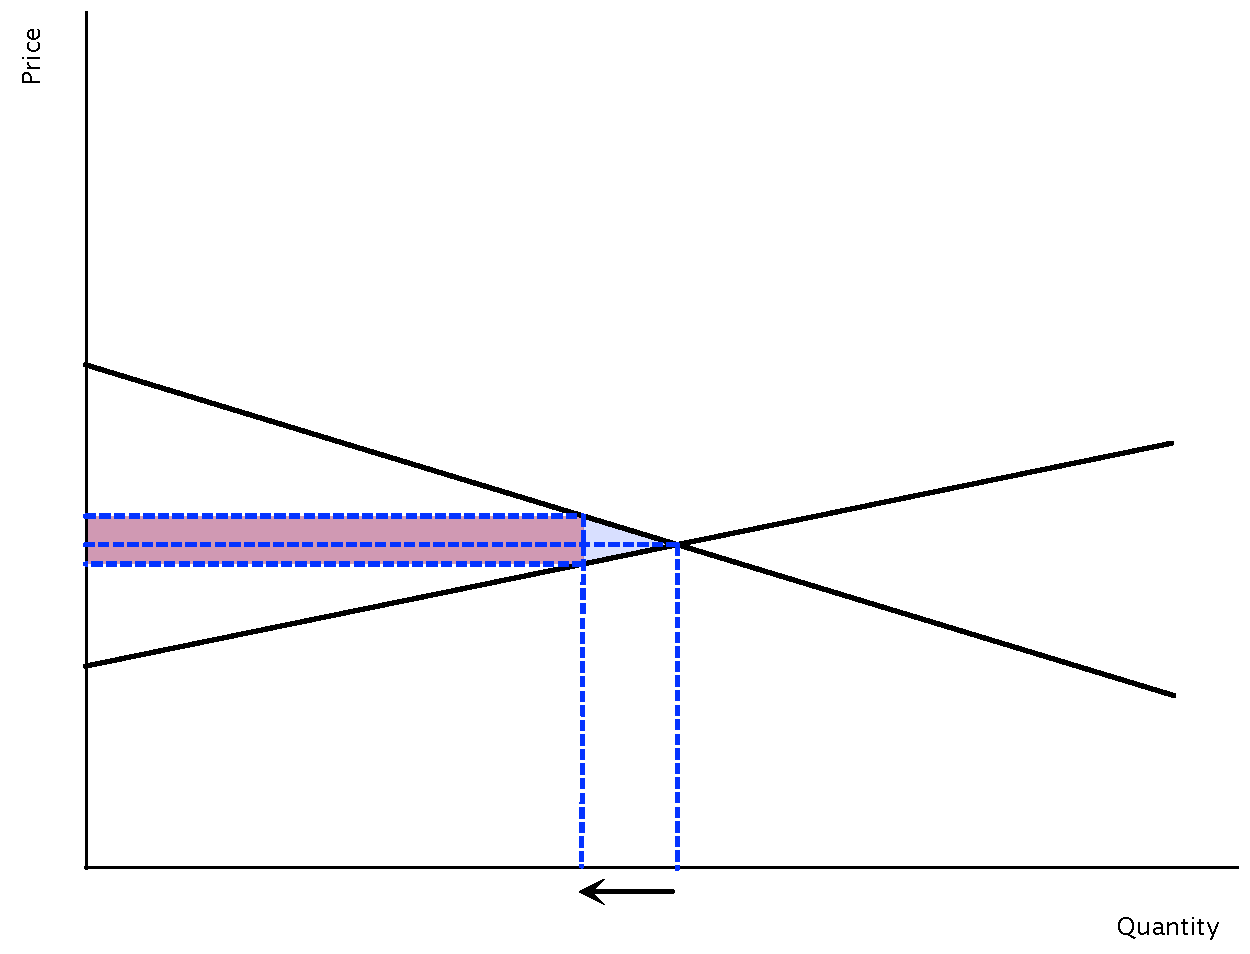
\includegraphics[scale=.15]{plot47.pdf}
			\caption{Small Tax}
		\end{subfigure}%
		\begin{subfigure}{.3\textwidth}
			\centering
			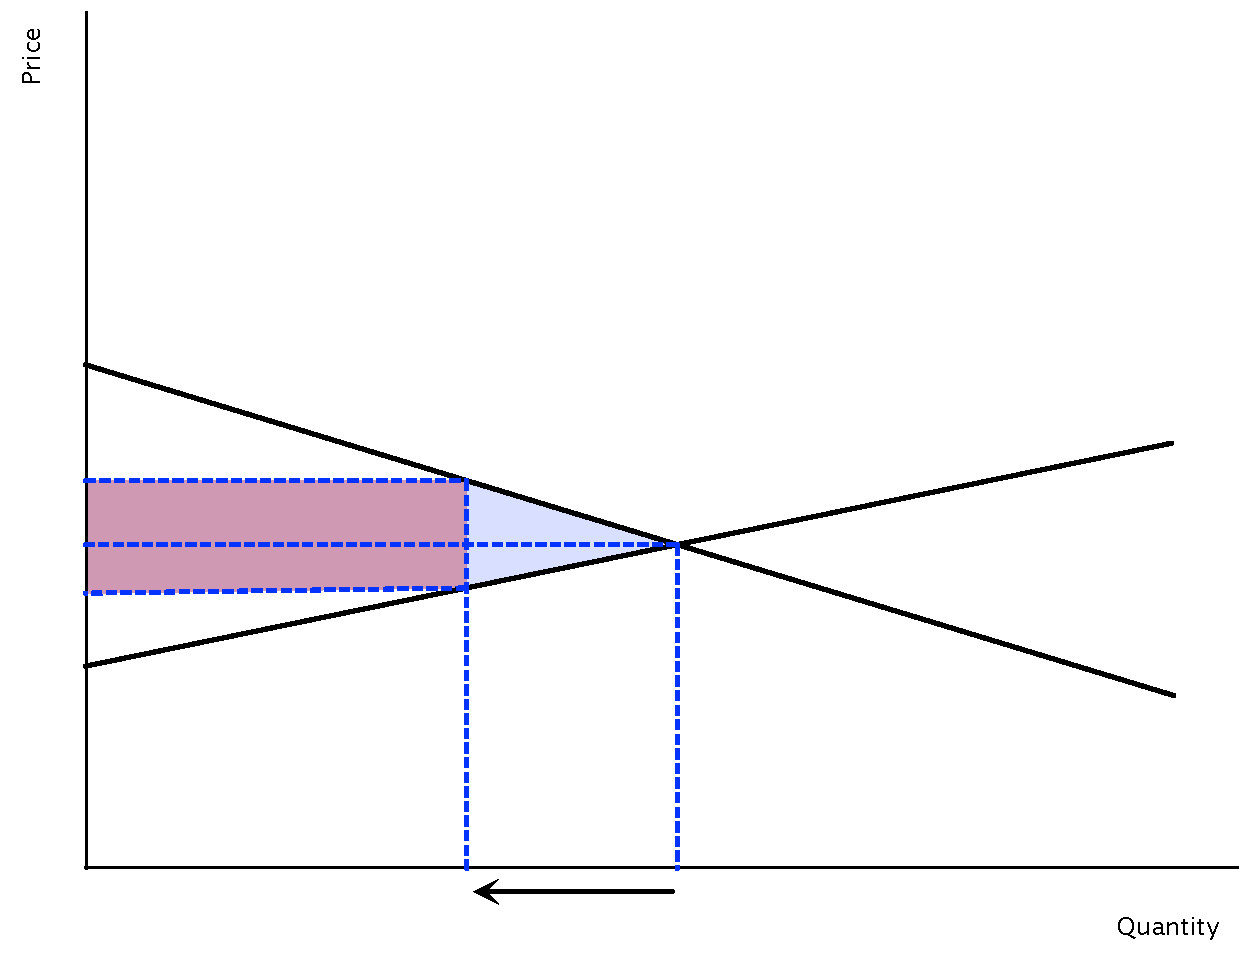
\includegraphics[scale=.15]{plot48.pdf}
			\caption{Medium Tax}
		\end{subfigure}
		\begin{subfigure}{.3\textwidth}
			\centering
			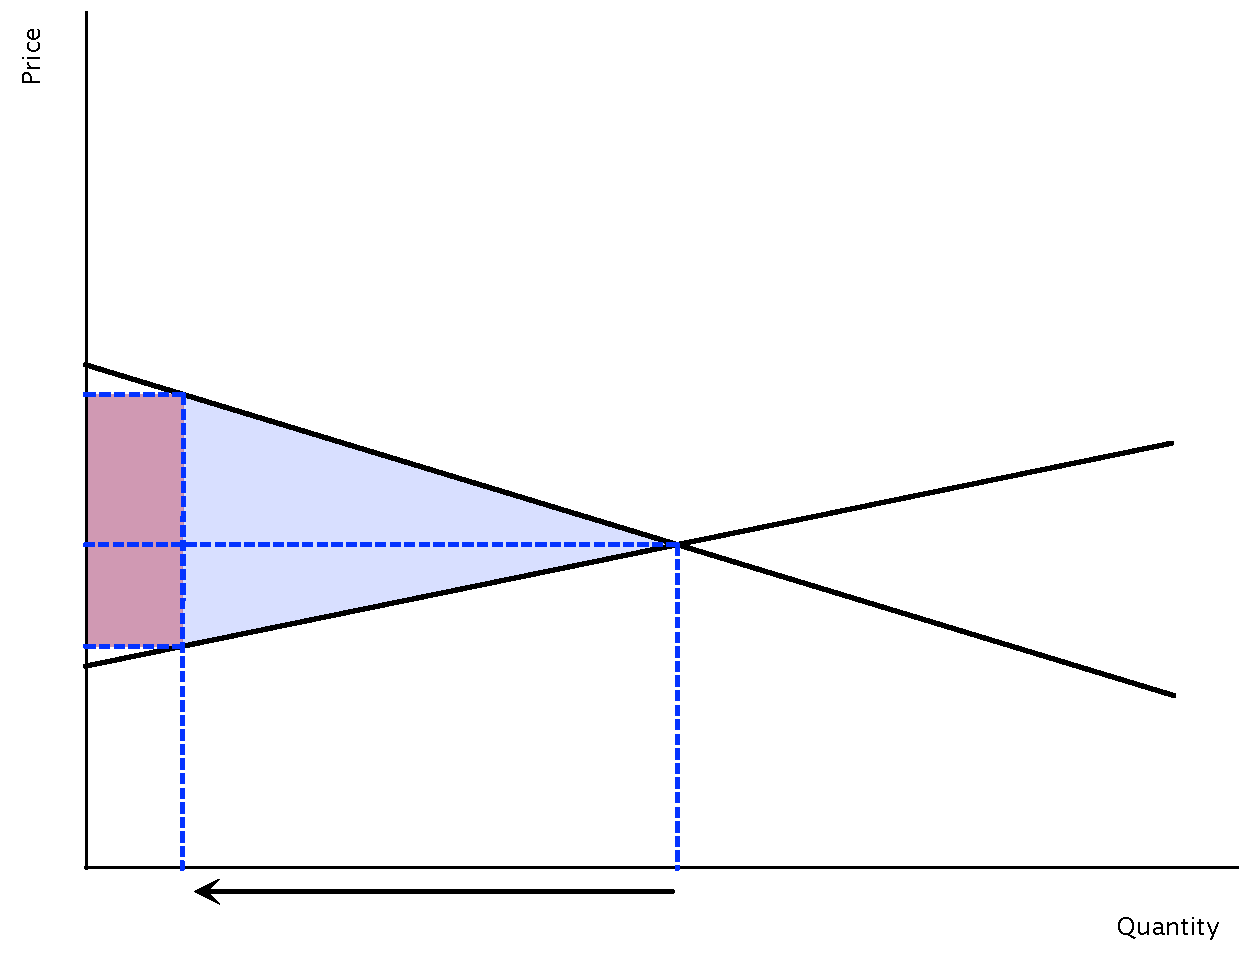
\includegraphics[scale=.15]{plot49.pdf}
			\caption{Large Tax}
		\end{subfigure}
	\end{figure} 
	
\end{frame}



\begin{frame}{Taxes}
	\begin{exmp}
		\scriptsize
		Table \ref{SA1} shows the willingness to pay and costs of six buyers and sellers in the market for headphones.
		
		\begin{table}[H]
			\caption{\scriptsize WTP and Seller Costs for Headphones}
			\centering
			\begin{tabular}{c|c} 
				
				WTP   & Seller Costs \\
				\hline
				\$200 & \$80 \\
				\$175 & \$120 \\
				\$160 & \$130 \\
				\$140 & \$140 \\
				\$120 & \$155 \\
				\$100 & \$180 \\
			\end{tabular}
			\label{SA1}
		\end{table}
		\begin{enumerate}[(a)]
			\item The government imposes a per-unit tax of \$55 on sellers of headphones. What will be the price buyers pay, the price sellers receive, and the quantity exchanged in the market as a result of this tax? 
			\item What is the tax revenue generated from this tax? The deadweight loss?
		\end{enumerate}
	\end{exmp}
\end{frame}

\section{Subsidies}

\begin{frame}{Subsidies}
	\begin{itemize}
		\item A (per unit) subsidy is just the reverse of a tax: The government provides buyers (or sellers) a dollar amount per-unit for the good 
		\item Similarly, subsidies have many of the same implications as per-unit taxes:
		\begin{enumerate}
			\item Subsidies drive a wedge between the price buyers pay and the price sellers receive
			\begin{itemize}
				\item Buyers pay a lower price than before
				\item Sellers receive a higher price than before
			\end{itemize}
			\item The split of the wedge depends on the relative elasticities of supply and demand
		\end{enumerate}
		\item Subsidies must be paid by taxpayers and create deadweight losses due to \textbf{inefficient transactions}
	\end{itemize}
	
\end{frame}



\begin{frame}{Subsidies}
	\begin{itemize}
		\item Much like taxes, the relative subsidy benefit between buyers and sellers depends on the elasticities of each curve
		\item The less elastic curve will realize a greater benefit from the subsidy as given by the difference between the new price received/paid and the old price
	\end{itemize}
\end{frame}

\begin{frame}{Subsidies}
	\begin{figure}[H]
		\centering
		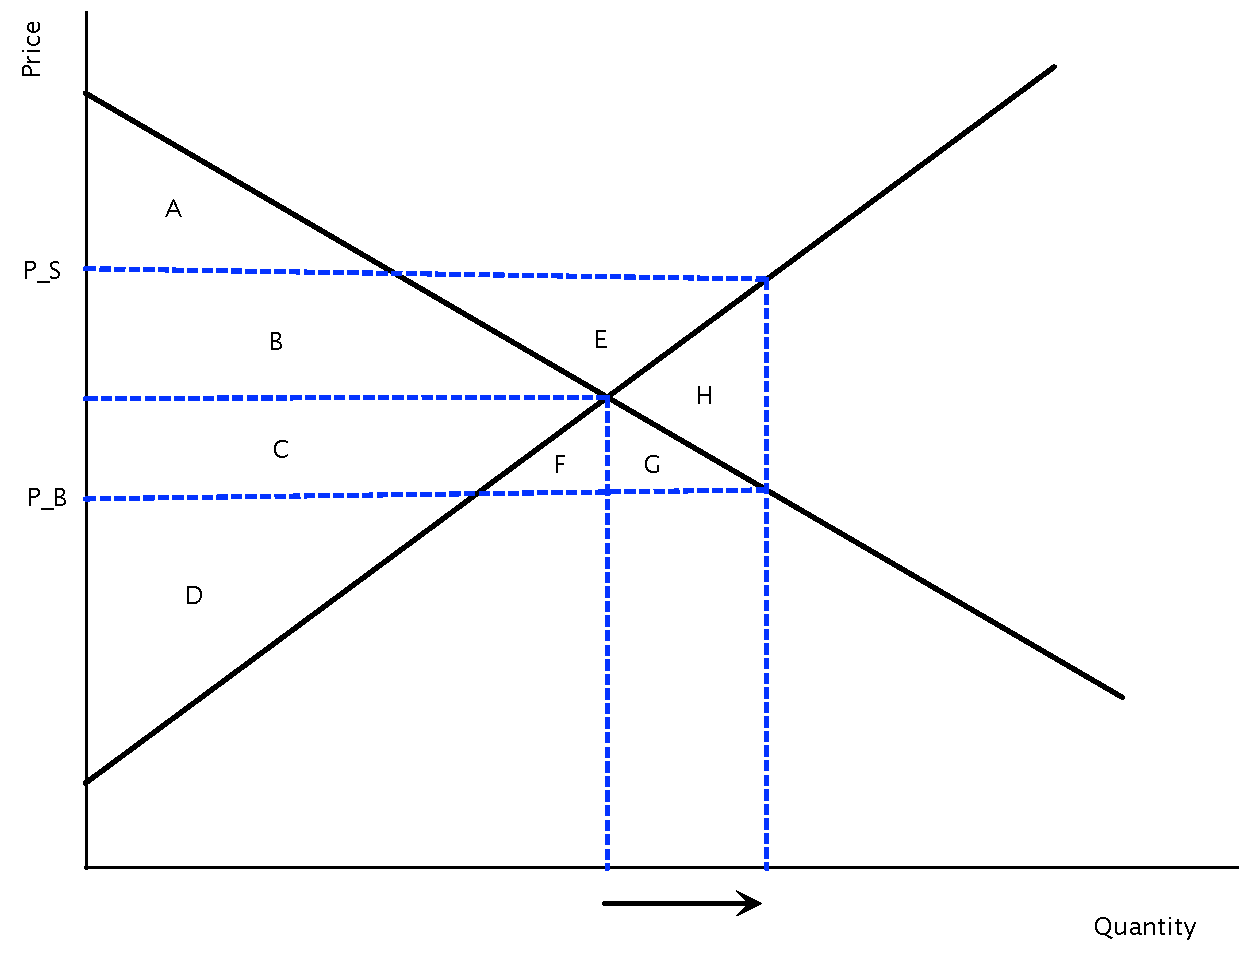
\includegraphics[scale=.3]{subsidy.pdf}
		\caption{Subsidies and Welfare}
	\end{figure}
\end{frame}

\begin{frame}{Subsidies}
	\begin{exmp}
		\scriptsize
		Consider the figure below, which shows the market for low-skilled labor. Suppose the government provides firms with a wage subsidy of \$4 per worker hired. How much will firms pay each worker? How much will each worker receive?

	\end{exmp}

	\begin{figure}[H]
	\centering
	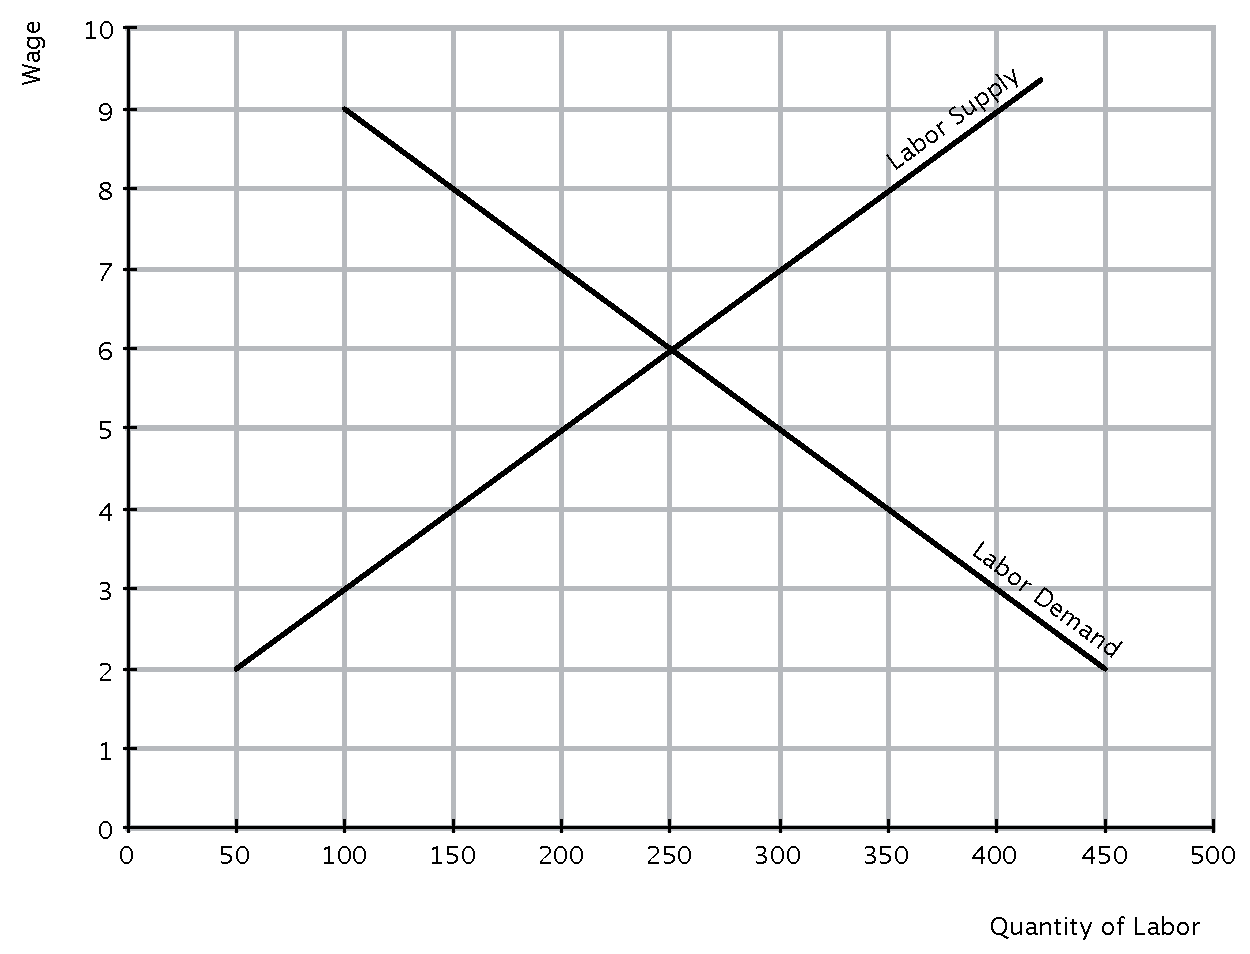
\includegraphics[scale=.3]{laborsubsidy.pdf}
	\caption{\scriptsize Labor Market}
\end{figure}

\end{frame}




\begin{frame}{Readings and Assignments}
\begin{itemize}
	\item Today: Mankiw Ch. 6, Ch. 8
	\item Next time: Mankiw Ch. 10, Ch. 11
	\item Problem Set 2, section 2 \& 3
\end{itemize}
\end{frame}

\end{document}